\documentclass[titlepage]{article}
\usepackage[margin=0.8in]{geometry}
\usepackage{tikz}
\usetikzlibrary{shapes.geometric, arrows, positioning}
\usepackage{hyperref}

\title{How to Clean the Keyboard of a Lenovo ThinkPad X200T}
\author{Jasper Chan -- 37467164}

\tikzstyle{startstop} = [
	rectangle,
	rounded corners,
	minimum width=3cm,
	minimum height=1cm,
	text centered,
	draw=black,
	fill=red!30
]

\tikzstyle{process} = [
	rectangle,
	minimum width=3cm,
	minimum height=1cm,
	text width=3cm,
	text centered,
	draw=black,
	fill=orange!30
]

\tikzstyle{decision} = [
	diamond,
	minimum width=3cm,
	minimum height=1cm,
	text width=3cm,
	text centered,
	draw=black,
	fill=green!30
]

\tikzstyle{truncatein} = [
	regular polygon,
	regular polygon sides=3,
	draw=black,
	font=\bfseries\Large
]

\tikzstyle{truncateout} = [
	regular polygon,
	regular polygon sides=3,
	shape border rotate=180,
	draw=black,
	font=\bfseries\Large
]

\tikzstyle{arrow} = [thick,->,>=stealth]

\begin{document}

\maketitle

\begin{figure}[p]
	\centering
	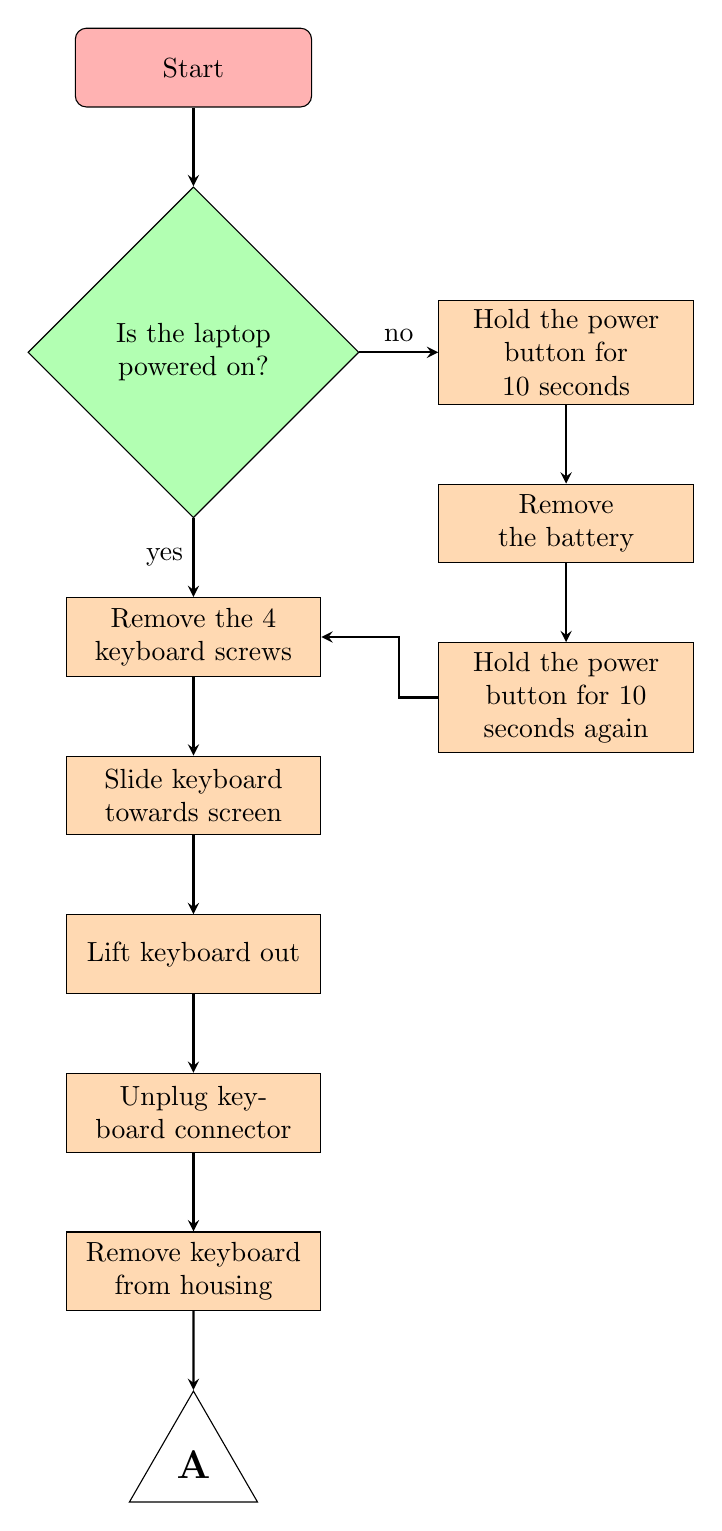
\begin{tikzpicture}[node distance=1cm]

		\node (start) [startstop] {Start};
		\node (ispower) [decision, below=of start] {Is the laptop powered on?};

		\node (holdpower1) [process, right=of ispower] {Hold the power button for 10 seconds};
		\node (removebattery) [process, below=of holdpower1] {Remove the battery};
		\node (holdpower2) [process, below=of removebattery] {Hold the power button for 10 seconds again};


		\node (removescrews) [process, below=of ispower] {Remove the 4 keyboard screws};
		\node (slideout) [process, below=of removescrews] {Slide keyboard towards screen};
		\node (liftkeyboard) [process, below=of slideout] {Lift keyboard out};
		\node (unplugkeyboard) [process, below=of liftkeyboard] {Unplug keyboard connector};
		\node (removekeyboard) [process, below=of unplugkeyboard] {Remove keyboard from housing};
		\node (truncatea) [truncatein, below=of removekeyboard] {A};

		\draw [arrow] (start) -- (ispower);

		\draw [arrow] (ispower) -- node[anchor=south] {no} (holdpower1);
		\draw [arrow] (holdpower1) -- (removebattery);
		\draw [arrow] (removebattery) -- (holdpower2);
		\draw [arrow] (holdpower2.west) -- +(-0.5,0) |- (removescrews);

		\draw [arrow] (ispower) -- node[anchor=east] {yes} (removescrews);
		\draw [arrow] (removescrews) -- (slideout);
		\draw [arrow] (slideout) -- (liftkeyboard);
		\draw [arrow] (liftkeyboard) -- (unplugkeyboard);
		\draw [arrow] (unplugkeyboard) -- (removekeyboard);
		\draw [arrow] (removekeyboard) -- (truncatea);
	\end{tikzpicture}
\end{figure}

\begin{figure}[p]
	\centering
	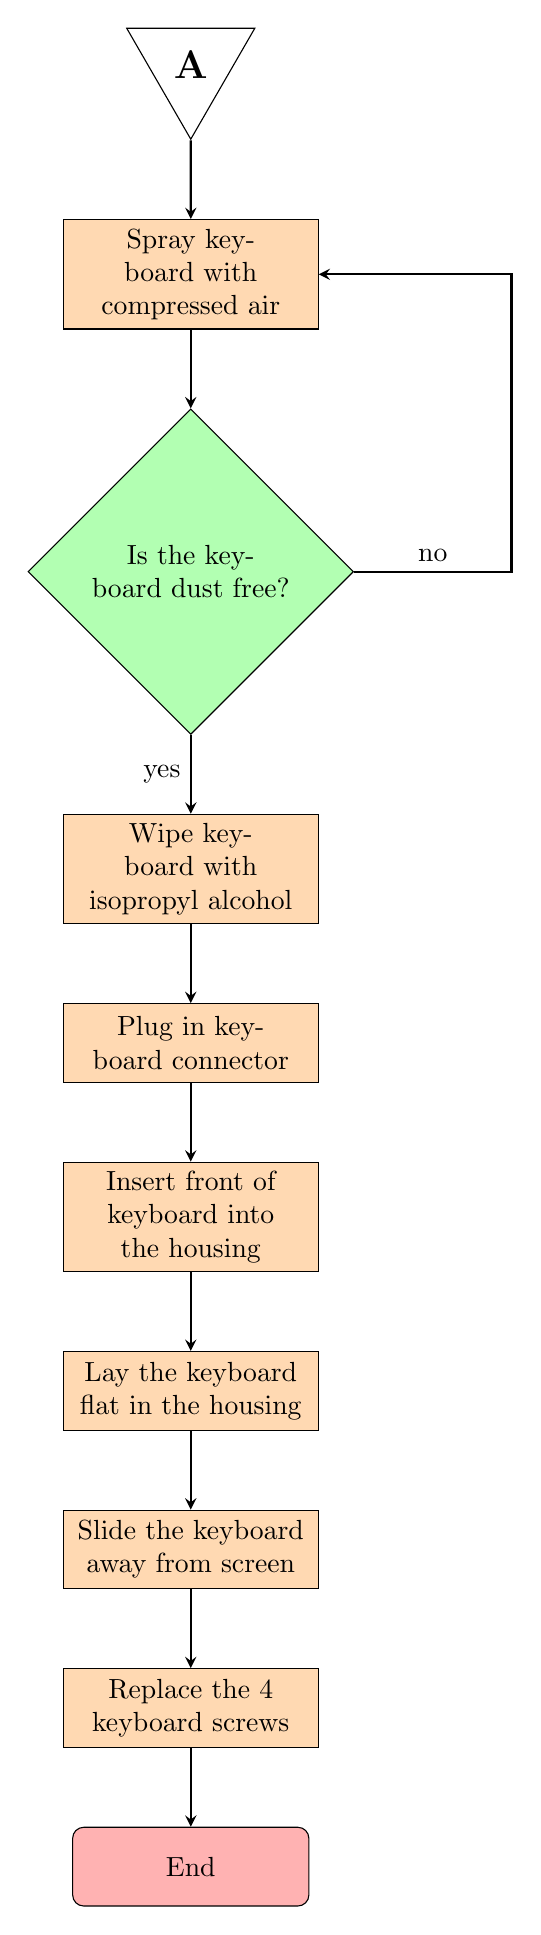
\begin{tikzpicture}[node distance=1cm]

		\node (truncatea) [truncateout] {A};

		\node (spraykeyboard) [process, below=of truncatea] {Spray keyboard with compressed air};
		\node (isclean) [decision, below=of spraykeyboard] {Is the keyboard dust free?};
		\node (wipekeyboard) [process, below=of isclean] {Wipe keyboard with isopropyl alcohol};
		\node (connectkeyboard) [process, below=of wipekeyboard] {Plug in keyboard connector};
		\node (insertkeyboard) [process, below=of connectkeyboard] {Insert front of keyboard into the housing};
		\node (flattenkeyboard) [process, below=of insertkeyboard] {Lay the keyboard flat in the housing};
		\node (slidein) [process, below=of flattenkeyboard] {Slide the keyboard away from screen};
		\node (replacescrews) [process, below=of slidein] {Replace the 4 keyboard screws};

		\node (end) [startstop, below=of replacescrews] {End};

		\draw [arrow] (truncatea) -- (spraykeyboard);

		\draw [arrow] (spraykeyboard) -- (isclean);
		\draw [arrow] (isclean.east) -- node [anchor=south] {no} +(2,0) |- (spraykeyboard.east);
		\draw [arrow] (isclean) -- node [anchor=east] {yes} (wipekeyboard);
		\draw [arrow] (wipekeyboard) -- (connectkeyboard);
		\draw [arrow] (connectkeyboard) -- (insertkeyboard);
		\draw [arrow] (insertkeyboard) -- (flattenkeyboard);
		\draw [arrow] (flattenkeyboard) -- (slidein);
		\draw [arrow] (slidein) -- (replacescrews);

		\draw [arrow] (replacescrews) -- (end);

	\end{tikzpicture}
\end{figure}


\end{document}
